\documentclass[a4paper, 12pt]{article}
\usepackage{cmap}
\usepackage{amssymb}
\usepackage{amsmath}
\usepackage{graphicx}
\usepackage{amsthm}
\usepackage{upgreek}
\usepackage{setspace}
\usepackage{color}
\usepackage[T2A]{fontenc}
\usepackage[utf8]{inputenc}
\usepackage[normalem]{ulem}
\usepackage{mathtext} % русские буквы в формулах
\usepackage[left=2cm,right=2cm, top=2cm,bottom=2cm,bindingoffset=0cm]{geometry}
\usepackage[english,russian]{babel}
\usepackage[unicode]{hyperref}
\newenvironment{Proof} % имя окружения
{\par\noindent{$\blacklozenge$}} % команды для \begin
{\hfill$\scriptstyle\boxtimes$}
\newcommand{\Rm}{\mathbb{R}}
\newcommand{\Cm}{\mathbb{C}}
\newcommand{\Z}{\mathbb{Z}}
\newcommand{\I}{\mathbb{I}}
\newcommand{\N}{\mathbb{N}}
\newcommand{\rank}{\operatorname{rank}}
\newcommand{\Ra}{\Rightarrow}
\newcommand{\ra}{\rightarrow}
\newcommand{\FI}{\Phi}
\newcommand{\Sp}{\text{Sp}}
\renewcommand{\leq}{\leqslant}
\renewcommand{\geq}{\geqslant}
\renewcommand{\alpha}{\upalpha}
\renewcommand{\beta}{\upbeta}
\renewcommand{\gamma}{\upgamma}
\renewcommand{\delta}{\updelta}
\renewcommand{\varphi}{\upvarphi}
\renewcommand{\phi}{\upvarphi}
\renewcommand{\tau}{\uptau}
\renewcommand{\lambda}{\uplambda}
\renewcommand{\psi}{\uppsi}
\renewcommand{\mu}{\upmu}
\renewcommand{\omega}{\upomega}
\renewcommand{\d}{\partial}
\renewcommand{\xi}{\upxi}
\renewcommand{\epsilon}{\upvarepsilon}
\newcommand{\intx}{\int\limits_{x_0}^x}
\newcommand\Norm[1]{\left\| #1 \right\|}
\newcommand{\sumk}{\sum\limits_{k=0}^\infty}
\newcommand{\sumi}{\sum\limits_{i=0}^\infty}
\newtheorem*{theorem}{Теорема}
\newtheorem*{cor}{Следствие}
\newtheorem*{lem}{Лемма}
\begin{document}
	\section*{Метод простой итерации}
	Дано уравнение $$2\sin 3x = x^2 - 4x+3.$$
	Отделить корень и привести к виду, удобному для итераций. Выбрать начальное приближение, обеспечивающее выполнение условий теоремы о сходимости метода простой итерации. Вычислить с точностью $\epsilon=10^{-2}$ корень уравнения.\\\\
	Приведем исходное уравнение к виду $f(x) = 0$: $$\underbrace{2\sin 3x - (x^2 - 4x+3)}_{f(x)} = 0.$$
	Область определения функции $f(x)$ совпадает с $\Rm$.
	Для начала построим графики для данного уравнения, так как в данном случае это легко сделать. Определим две функции $$y = 2\sin 3x,\quad y = x^2 - 4x+3$$ и построим их графики.
	$$
		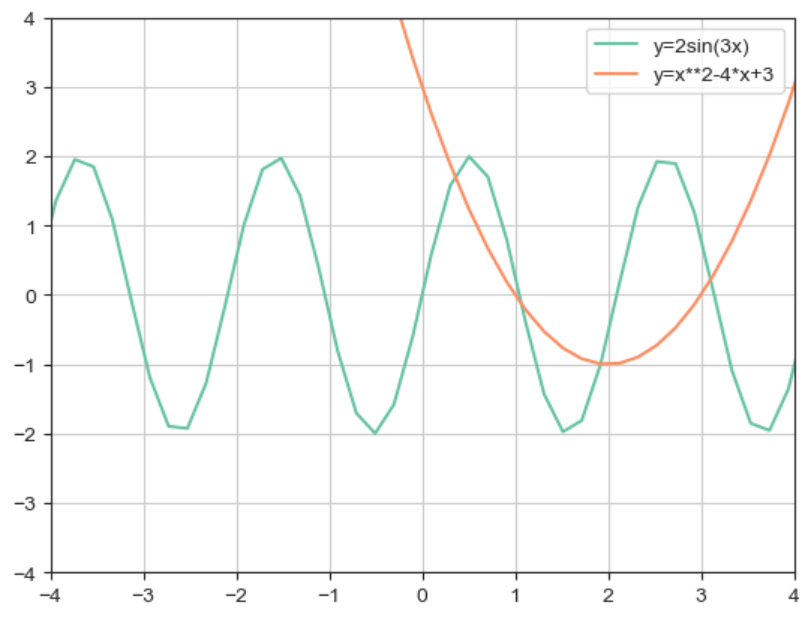
\includegraphics[scale=0.7]{img1}
	$$
	Таким образом, уравнение $f(x)=0$ имеет 4 корня. Будем вычислять корень, который находится \textit{левее всех} на графике. Его мы и будем отделять. \\\\
	\textbf{Отделение корня}. По графику мы можем понять, что нужный нам корень лежит где-то на отрезке $[0, 0.5]$. Покажем, что на этом отрезке действительно есть только один корень нашего уравнения. Воспользуемся теоремой:\\\\
	\textbf{Теорема.}
		\textit{Если функция $f(x)\in C[a,b]$ и принимает на его концах значения разных знаков, то на этом отрезке существует по крайней мере один корень уравнения $f(x) = 0$.
		Если при этом функция $f(x)$ будет монотонной на отрезке $[a,b]$, то она может иметь только один корень.}
	\begin{enumerate}
		\item Покажем \textit{существование}: вычислим значения на концах отрезка
		$$f(0) = -3,\quad f(0.5) = 0.745 \quad\Rightarrow\quad f(0) < 0 < f(0.5)$$
		То есть, действительно на $[0, 0.5]$ есть корень уравнения, т.к. значения разных знаков.\\\\
		\textbf{В случае, если знаки окажутся одинаковыми}, необходимо сделать несколько шагов деления отрезка пополам (дихотомии). Пусть мы изначально взяли отрезок $[0, 1.5]$. В этом случае, как можно увидеть на графике, мы случайно захватили еще один корень и при этом $$f(1.5)=-1.21 \quad \Rightarrow\quad f(0) < f(1.5) < 0.$$ Для отделения корней поделим отрезок пополам, то есть $$[0, 1.5] = [0, 0.75] \cup [0.75, 1.5]$$ и рассмотрим значение в новой точке $$f(0.75) = 0.993 > 0  \quad \Rightarrow\quad f(0) < 0<f(0.75),$$ что нам и требовалось. В ином случае пришлось бы делать еще шаги деления отрезка. Таким образом, мы проделали \textit{одну итерацию дихотомии.} 
		\item  Покажем \textit{единственность}:
		$$f'(x) = 6\cos 3x - (2x - 4) > 0 \quad \forall x \in [0, 0.5],$$
		то есть $f(x)$ является монотонно возрастающей, т.к. первая производная не меняет знак.
		Действительно $$
		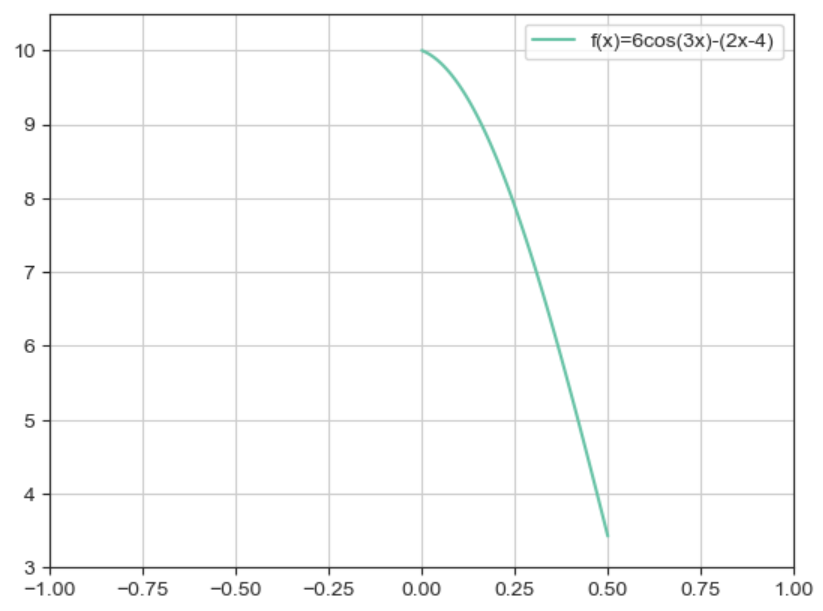
\includegraphics[scale=0.7]{img2}
		$$
		(график производной необязателен). Значит корень на $[0, 0.5]$ всего один. \\\\
		\textbf{В случае, если первая производная меняет знак}, то это еще не значит, что корень на отрезке не единственный. Для примера возьмем отрезок $[0, 0.75]$. Ранее мы выяснили, что на этом отрезке существуют корни $f(x) = 0$. Но поскольку $f'(0) > 0$, $f'(0.75) < 0$, то $f'(x)$ на этом отрезке меняет знак. Тогда вычислим вторую производную $$f''(x) = -18\sin(3x) - 2 < 0 \quad \forall x \in [0, 0.75].$$ Вторая производная не изменяет знак, и этого достаточно для того, чтобы функция была монотонна. Поэтому на отрезке $[0, 0.75]$ также один корень. 
	\end{enumerate}
	\textbf{Приведем уравнение к виду, удобному для итераций}, т.е. к виду $x = \varphi(x)$. Одним из способов является приведение уравнения к виду $$x = \underbrace{x - \lambda f(x)}_{\varphi(x)},\quad \lambda = \dfrac{1}{\max_{x\in[a,b]}|f'(x)|},$$
	причем мы \textit{гарантировано получим сходящийся итерационный процесс}.
	Вычислим $\lambda$: (исходя из графика) $$|f'(x)| = |6\cos 3x - (2x - 4)| \leq |f'(0)| = 10.$$ Значит $$\lambda = \dfrac{1}{10} = 0.1$$
	и $$x = \underbrace{x - 0.1\cdot (2\sin 3x - (x^2 - 4x+3))}_{\varphi(x)}.$$
	Отсюда итерационный процесс будет определяться формулой $$x_{k+1} = x_k - 0.1\cdot (2\sin 3x_k - (x_k^2 - 4x_k+3)).$$
	\textbf{Выберем начальное приближение.} К примеру возьмем левый край нашего отрезка $[0, 0.5]$, то есть $$x_0 = 0.$$
	Мы также могли бы взять и правый край отрезка, и его центр или любую другую точку из отрезка.\\\\
	\textbf{Проверим выполнение условий теоремы о сходимости} МПИ: 
	\begin{theorem}
		[о сходимости метода простой итерации]
		Пусть выполняются следующие условия:\begin{enumerate}
			\item функция $\varphi(x)$ определена на отрезке $$|x - x_0| \leq \delta,\eqno(3)$$ непрерывна на нем и удовлетворяет условию Липшица с постоянным коэффициентом меньше единицы, то есть $\forall x, \widetilde{x}$ $$|\varphi(x) - \varphi(\widetilde{x})| \leq q |x - \widetilde{x}| ,\quad 0 \leq q < 1;\eqno(4)$$
			\item для начального приближения $x_0$ верно неравенство $$|x_0 - \varphi(x_0)| \leq m;$$
			\item числа $\delta, q, m$ удовлетворяют условию $$\dfrac{m}{1-q}\leq \delta. \eqno(5)$$
		\end{enumerate}
		Тогда \begin{enumerate}
			\item уравнение $x = \varphi(x)$ в области $(3)$ имеет решение;
			\item последовательность $x_k$ построенная по правилу $x_{k+1} = \varphi(x_k)$ принадлежит отрезку $[x_0 - \delta, x_0 + \delta]$, является сходящейся и ее предел удовлетворяет уравнению $x = \varphi(x)$.
		\end{enumerate}
	\end{theorem}
	Будем идти последовательно по пунктам теоремы. 
	\begin{enumerate}
		\item Выберем произвольно $\delta = 0.5$. Поскольку $x_0 = 0$, то для выполнения условия необходимо, чтобы на отрезке $$[x_0 - \delta; x_0 + \delta] = [-0.5; 0.5]$$ функция $\varphi(x)$ была определена и непрерывна. Очевидно это выполняется, т.к. $\varphi(x) = x - 0.1\cdot (2\sin 3x - (x^2 - 4x+3))$ определена и непрерывна на $\Rm$.\\\\
		Выполнение условия Липшица можно заменить равносильным ему условием $$|\varphi'(x)| \leq q.$$
		Отсюда остается лишь найти значение $q$: $$|\varphi'(x)| = |1 - 0.6\cos3x + 0.2x - 0.4| \leq |\varphi'(0.5)| \approx 0.658.$$
		Таким образом, выбираем $q = 0.658$, а значит условие выполнено.
		\item Из неравенства найдем значение $m$: $$|x_0 - \varphi(x_0)|  =|0-\varphi(0)| = |0- 0.3| = 0.3.$$
	Отсюда выбираем $m=0.3$.
	\item Проверяем, выполнилось ли неравенство (5): $$\dfrac{0.3}{1-0.658} \approx 0.0877 < 0.5.$$
	\end{enumerate}
	Условия теоремы выполнены, значит итерационный процесс действительно сойдется к некоторому решению при заданной точности. \\\\
	\textbf{В случае, если условия теоремы не были выполнены}, то можно попробовать взять другое начальное приближение $x_0$, а также попробовать задать другое $\delta$.\\\\
	\textbf{Вычислим корень} уравнения с заданной точностью $\epsilon=10^{-2}$. Выпишем еще раз формулы для итерационного процесса:
	$$\begin{cases}
		x_{k+1} = x_k - 0.1\cdot (2\sin 3x_k - x_k^2 + 4x_k-3),\\
		x_0 = 0.
	\end{cases}$$
	Будем делать итерации, пока $$|x_{k+1} - x_k| > \epsilon.$$
	Легко вычислить $$x_1 = x_0 - 0.1\cdot (2\sin 3x_0 - x_0^2 + 4x_0-3) = -0.1\cdot(-3) = 0.3 \quad \Rightarrow \quad |0.3 - 0| = 0.3 > 0.01.$$
	$$x_2 \approx 0.332 \quad \Rightarrow \quad |0.332 - 0.3| = 0.032 > 0.01.$$
	$$x_3 \approx 0.342 \quad \Rightarrow \quad |0.342 - 0.332| = 0.012 > 0.01.$$
	$$x_4 \approx 0.346 \quad \Rightarrow \quad |0.346 - 0.342| = 0.004 < 0.01.$$
	Таким образом, получаем приближенный корень $x \approx 0.346$.
\end{document}